% !TEX root = praca.tex

\chapter{Architektura systemu}
\label{cha:architekturaSystemu}

Napisać coś o tym, że całość architektury zawiera wiele integracji, używa kilka protokołów komunikacyjnych itp.
Dobra architektura systemu powinna zapewnić łatwe skalowanie oraz utrzymanie. Należy zrozumieć wymagania zarówno funkcjonalne czyli jakie zadania system ma spełniać, oraz niefunkcjonalne czyli wydajność lub bezpieczeństwo. Innym ważnym aspektem jest podział odpowiedzialności czyli na jakie komponenty powinien zostać podzielony system.

Zdecydowano, że autonomiczny system kompletacji zamówień musi zostać podzielony na trzy aplikacje: aplikacja internetowa, aplikacja serwerowa oraz aplikacja sterowania robotem. Taka architektura zapewniła odpowiedni podział odpowiedzialności na warstwę prezentacji, warstwę logiki biznesowej i warstwę zarządzania i sterowaniem robotem. Dzięki temu wszystkie trzy systemy można rozwijać niezależnie. Dodatkowo taki podział umożliwia wykorzystanie wielu robotów, poprzez odpowiednią integrację z aplikacją serwerową. Podział na trzy aplikacje można zobaczyć na rysunku \ref{fig:c4Modelc1}, który przedstawia poziom C1 w modelu C4 architektury systemu.

Może coś o procesie decyzyjnym, jakie inne zalety ma to rozwiązanie, albo jakie wady lub ograniczenia. Zaletą jest to że aplikacja frontendowa nie komunikuje się bezpośrednio z robotem. 

\begin{figure}[htbp]
    \centering
    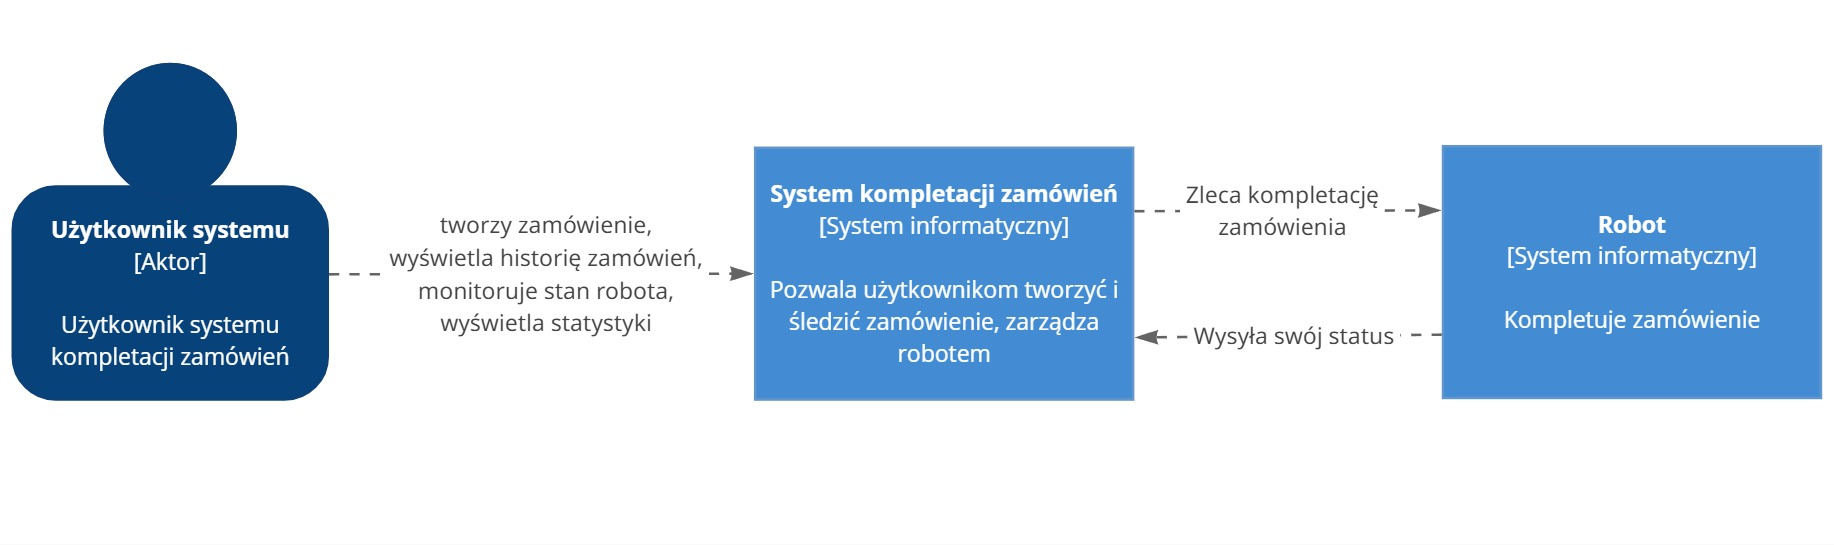
\includegraphics[width=1\textwidth]{images/c4_architecture-C1.jpg}
    \caption{Model C4 architektury systemu - poziom C1}
    \label{fig:c4Modelc1}
\end{figure}

%---------------------------------------------------------------------------

\section{Integracje aplikacji i usług}
\label{sec:integracje}

Ogólnie opisać komunikację między poszczególnymi systemami projektu.
Podział na trzy niezależne aplikacje wymaga zaprojektowania odpowiedniej komunikacji między nimi. Jednak każdy z systemów ma inne odpowiedzialności i wymagania co wymagało zastosowania różnych mechanizmów komunikacji.

%---------------------------------------------------------------------------

\subsection{Komunikacja aplikacji internetowej i serwerowej}
\label{sec:komunikacjaBackendFrontend}

Opisać http (rest api) i web sockety
Główną odpowiedzialnością aplikacji internetowej jest integracja z użytkownikiem, który może wyświetlić listę produktów, stworzyć zamówienie czy wyświetlić historię zamówień. Najlepszym wyborem dla operacji inicjowanych przez użytkownika, które polegają na wysłaniu żądania i otrzymaniu odpowiedzi jest REST. Coś napisać o REST API.

Użytkownik oprócz wysyłania pojedycznych żądań powinien móc śledzić swoje zamówienie. Jednak ciągłe odświeżadanie strony lub cykliczne wysyłanie zapytań do serwera o stan robota nie jest najlepszym wyborem. Dlatego zdecydowano się na SignalR, technologię która wykorzystuje WebSockety. i coś tam coś tam co umożliwia stałe połączenie z serwerem i komunikację w czasie rzeczywistym (czy na pewno rzeczywistym???). i coś tam coś tam że serwer przesyła dane o stanie robota, gdzie się znajduje, jakie produkty zebrał, ile trwa zamówienie itd.

%---------------------------------------------------------------------------

\subsection{Komunikacja robot - backend}
\label{sec:komunikacjaRobotBackend}

Opisać mosquitto

%---------------------------------------------------------------------------

\section{nie wiem}
\label{sec:integracjecd}
To z jakich aplikacji oraz usług składa się system oraz jak one się ze sobą komunikują doskonale widać na diagramie poziomu C2 modelu C4 architektury systemu, który został przedstawiony na rysunku \ref{fig:c4Modelc2}.

\begin{figure}[htbp]
    \centering
    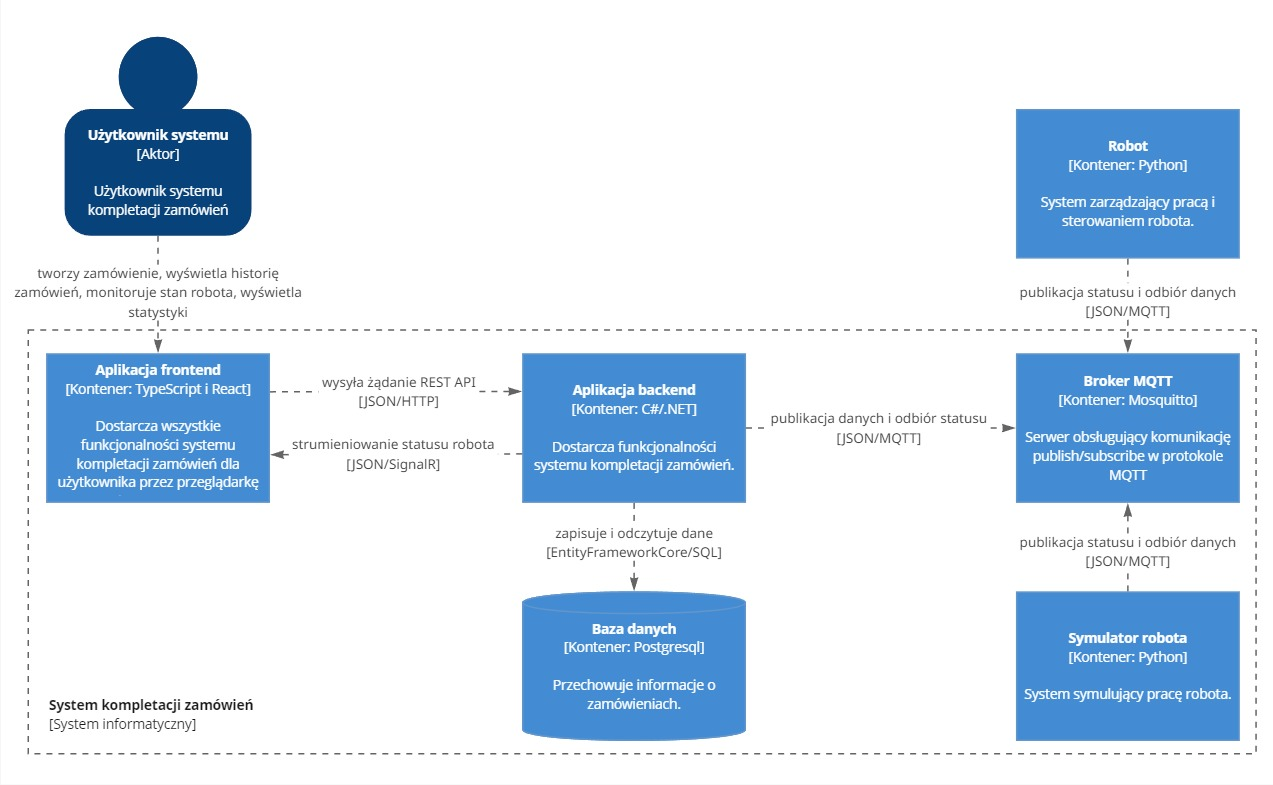
\includegraphics[width=1\textwidth]{images/c4_architecture-C2.jpg}
    \caption{Model C4 architektury systemu - poziom C2}
    \label{fig:c4Modelc2}
\end{figure}